\documentclass[11pt]{article}

\usepackage[T1]{fontenc}
\usepackage[margin=1in]{geometry}
\usepackage{amsmath}
\usepackage{amssymb}
\usepackage{booktabs}
\usepackage{array}
\usepackage{tabularx}
\usepackage{longtable}
\usepackage{xcolor}
\usepackage{caption}
\usepackage{microtype}
\usepackage{enumitem}
\usepackage{tikz}
\usetikzlibrary{arrows.meta,positioning,fit,calc}
\usepackage{pgfplots}
\pgfplotsset{compat=1.16}
\usepackage[colorlinks=true,linkcolor=blue!45!black,citecolor=blue!45!black,urlcolor=blue!45!black]{hyperref}

\hypersetup{pdftitle={Monet v1.0},pdfauthor={Allen Hsieh}}

\captionsetup{font=small, labelfont=bf}
\setlist{itemsep=2pt, topsep=4pt}

% Float packing: let tables share pages with more text instead of drifting.
\renewcommand{\topfraction}{0.9}
\renewcommand{\bottomfraction}{0.6}
\renewcommand{\textfraction}{0.07}
\renewcommand{\floatpagefraction}{0.8}
\setcounter{totalnumber}{4}
\setcounter{topnumber}{3}

\newcommand{\code}[1]{\texttt{#1}}
\newcommand{\usff}{\code{us54}}
\newcommand{\monet}{MONET.md}
\newcommand{\sect}[1]{\S#1}

% ---- the acceptance read's numbers (MONET.md 3.8ba), set once here --------------------------------------
\newcommand{\VSestMeanPct}{$58.38\%$}
\newcommand{\VAcceptOutcome}{all six met, condition 5 as registered: v1.0 is v0.54's vector}
\newcommand{\VWallHours}{one and a half}
\newcommand{\VPinsTwin}{$12$ of $12$}
\newcommand{\VCsixRead}{$58.3819\%$ against $58.3819\%$, every seed equal; $14{,}400$ of $14{,}400$ games byte-identical}
\newcommand{\VCsixVerdict}{met}
\newcommand{\VCsixPara}{The second adapter was built independently at \sect{3.8m}: its view builder is its own, and it shares only the policy it wraps. It played SESTINA on the same twelve seeds from the same tree. Its win rate equals the arm's to four decimals on every seed ($58.3819\%$ pooled on both), every other engine line is equal on every cell, and all $14{,}400$ games are byte-identical when matched on deal and rotation; the engine's own count of Monet's asks is identical on $12$ of $12$ cells. At v0.33's vector the twin had differed on $4$ games of $14{,}400$, all at one position that changed no result (\sect{3.8at}); here no game differs.}
\newcommand{\VPredScore}{All six held, so each prediction hit, condition 5 by the registration's rules rather than by its reader's line. One read cannot say whether $45\%$ was well calibrated. It does say that the doubt the registration placed on condition 3 did not materialise: SESTINA sat $0.15$ points above v0.6, not more than the floor.}

\title{Monet v1.0: imitating a frontier Canadian Fish agent, correcting the imitation, and passing a
pre-registered acceptance test}
\author{Allen Hsieh\\[2pt] {\small FishAI project}}
\date{September 2026}

\begin{document}
\maketitle

\begin{abstract}
\noindent Monet is an agent for Canadian Fish, the six-player team card game, under the \usff{} rules.
It began on 2026-09-01 as FishAI's Bass v2.0, which won $27.08\%$ of its games against SESTINA v1.0,
the frontier agent of the FishLab lineage, and it climbed through fifty-five rungs, each registered
before it was measured and each measured against SESTINA in FishLab's own engine. Version 1.0 was
defined in advance by six conditions rather than by a date. The vector that meets them asks with a
small network that imitates SESTINA's choice, overruled by a second network trained on paired
play-outs of what wins; its belief is hand-built constraint tracking with a fitted card-by-seat table,
its declarations are hand-written, and it searches nothing at play time. On the acceptance read it won
$58.38\%$ of $14{,}400$ games against SESTINA on twelve fresh seeds, with no seed below $56.58\%$; it
beat each of five earlier FishLab agents; it declared correctly on at least $99.49\%$ of attempts in
every cell; and an independently built adapter reproduced all $14{,}400$ of its games against SESTINA byte for byte. We report the rungs that failed as fully as those that shipped: no
play-time search beat the agent it searched over against SESTINA, and a search over every legal ask on
Monet's own belief was worth $-0.14$ sets at a decision against a hindsight ceiling of $+2.84$. We also
report that the read's locked control reader printed ``not met'', and how the registration's own rules
decide it.
\end{abstract}

\section{Introduction}
\label{sec:intro}

Canadian Fish is a game of asking. Six players in two teams of three hold a shuffled deck; on a turn a
player asks one opponent for one card, and keeps the turn while the asks hit. A team scores a
half-suit by declaring, from memory and inference, which teammate holds each of its six cards, and a
wrong declaration hands the set to the other side. The information is public but scattered across a
long log, the hands change with every hit, and the value of an ask lies less in the card than in what
it reveals and what it sets up.

This paper is the final report on Monet, the agent line FishAI built to answer one question the
project's owner set on 2026-09-03 and sharpened on 2026-09-10: can a FishAI agent be \emph{consistently}
better than SESTINA v1.0? SESTINA is the frontier agent of FishLab \cite{fishlab}, an independent
engine and bot family whose C++ engine plays a guest bot over a JSON protocol. Every number in this
paper is a game played on that engine, against that opponent, through a bridge described in
\sect\ref{sec:bridge}; FishAI's own engine is used only as a cheap screen.

\paragraph{How the work was done.} Monet was built as a ladder. Each rung wrote its mechanism, the bar
that would ship it, a probability for each prediction, and its cost into the project's research record,
\monet{} \cite{monet}, before the first game was played, and each rung's outcome was recorded whether
or not it shipped. Twelve vectors shipped. Most rungs did not, and the record of why is the bulk of what
the project learned (\sect\ref{sec:negatives}).

\paragraph{What the paper reports.}
\begin{enumerate}
  \item \emph{The agent} (\sect\ref{sec:agent}): a belief built from constraints and a fitted table, a
        hand-written ranker whose numbers become features, a clone of SESTINA's asks, and a learned
        advantage that overrules the clone when it expects more than $0.05$ sets from another ask.
  \item \emph{The ladder} (\sect\ref{sec:ladder}): from $27.08\%$ to $58.42\%$ against SESTINA in four
        phases --- belief, ranker terms, imitation, and the learned correction.
  \item \emph{The negatives} (\sect\ref{sec:negatives}): six forms of play-time search, the belief after
        v0.4c, and the selectors over the clone's shortlist, all measured and all at or below zero.
  \item \emph{The game} (\sect\ref{sec:findings}): what the records say about Fish between strong agents,
        beginning with the exchange rate of one set a game for $12.8$ points of win rate.
  \item \emph{The acceptance read} (\sect\ref{sec:accept}): the six conditions at v0.54's vector, on
        $100{,}800$ games, with the one condition whose locked reader disagreed set out in full.
  \item \emph{The comparison} (\sect\ref{sec:compare}) with Bass v2.0, SESTINA v1.0 and Kraken v1.0, and
        the limits of every claim here (\sect\ref{sec:limits}).
\end{enumerate}
Writing the paper found errors in our own record; \sect\ref{sec:errata} lists them and where \monet{}
now corrects them.

\section{The game, the opponent and the bridge}
\label{sec:setting}

\subsection{Canadian Fish under \usff}

Canadian Fish (Literature) is a six-player game of two teams of three, seated alternately. \usff{}
\cite{rules} is the ``US student'' dialect FishAI plays: all $54$ cards (the standard deck with the
eights and two distinguishable jokers) are dealt, nine to a player, and form nine half-suits of six ---
low and high in each suit, plus a ninth of the four eights and the two jokers. On a turn a player asks
one opponent for one specific card, and may ask only for a card of a half-suit in which they hold at
least one card and do not hold the card asked for. A hit transfers the card face up and the asker asks
again; a miss passes the turn to the player who was asked. At any time, in or out of turn, a player may
\emph{declare} a half-suit by naming the teammate who holds each of its six cards. A fully correct
declaration scores the set for the declarer's team; \emph{any} error --- an opponent holding one of the
six, or a card assigned to the wrong teammate --- scores it for the opponents. The game ends the moment
a team has five sets, so ties cannot occur. Card counts and the full log of asks, answers and declares
are public; the hands are not.

Three consequences of these rules shape everything below. \emph{Every ask is evidence}: the asker has
revealed a card of the half-suit (the \emph{licence}), and a miss proves the target lacks the card.
\emph{A wrong declaration is a two-set swing}: the set a correct declaration would have scored goes to
the other side instead. \emph{A set the team fully holds is safe}: the opponents hold none of it and can
never ask into it, so a certain set loses nothing by waiting.

\subsection{The opponent: SESTINA v1.0 and the panel}

SESTINA v1.0 is the frontier agent of the FishLab project \cite{fishlab}, which publishes a C++ engine,
a family of bots and an evaluation laboratory for the same game. Every number in this paper is Monet
playing SESTINA's frozen release specification, verified byte-identical to the release asset
(\monet{} \sect{6.1}):
\begin{center}
\small\code{v07:r12=25,rtie=1,pool=-1,oppfloor=-1,force=1000000,askfloor=-1,stall=12,}\\
\small\code{s1=1,det=12,cand=4,kappa=2.5,rbelief=indep,depth=12,maxq=26}
\end{center}
From FishLab's documentation and engine source (read for facts, restated here in our own words):
SESTINA chooses an ask by a linear score over twenty features of each legal ask, with weights fitted by
cross-entropy search, and a one-step lookahead over that score. The keys \code{s1}, \code{det},
\code{cand}, \code{depth}, \code{kappa} and \code{maxq} configure a determinized search that runs only
in the endgame, when at most $26$ cards are unresolved: it samples $12$ deals consistent with the
public record, plays each of the top $4$ candidate asks out $12$ moves under a blueprint policy (whose
belief \code{rbelief} names), and departs from the blueprint's own pick only when a candidate beats it
by $2.5$ paired standard errors. It declares a set when its team-ownership probability for the plan
is at least $0.849$ and a value check agrees; on our records it declared with cards it could not place
$0.53$ times a game, right $84.1\%$ of the time (\monet{} \sect{3.8aj}).

The \emph{panel} is FishLab's earlier releases v0.2 to v0.6, which neither adapt nor, from v0.5 on,
search. They are in the acceptance test for one reason, stated when it was written: a bot that beats
SESTINA and loses to v0.5 ``has been fitted, not built'' (\monet{} \sect{3.9}).

\subsection{The bridge}
\label{sec:bridge}

Monet is measured \emph{abroad}: FishAI's decision function is installed as a guest bot inside
FishLab's engine and speaks its documented JSON-lines protocol through an adapter that builds FishAI's
public view from the host's events. FishLab's repository carries no licence file, so the engine, the
recording fork, the adapters and the game records live outside FishAI's public repository and nothing
of FishLab's is reproduced here; its game output is data, and its measured findings are cited as its
own. Two dialect differences are translated at the adapter, never in the policy. \usff{} has no pass,
and the host offers one to a turn-holder with no cards (PASSFIX: take it). \usff{} compels a declaration
when every opponent is out of cards, and the host offers an optional poll instead (MUSTFIX, adopted on
2026-09-04: an uncertain compelled claim is answered \code{none} and the host's own forced endgame
resolves it; worth $+1.28$ points paired on v0.9's vector, ahead on 12 of 12 seeds, \monet{}
\sect{3.8f}). The host plays all nine half-suits where \usff{} stops at five; the winner is the same.

\paragraph{Cells, reads and floors.} A \emph{cell} is one seed: $200$ duplicate deals, each played in
all $6$ seat rotations, $1{,}200$ games. A \emph{read} is twelve cells on fresh seeds, $14{,}400$ games,
quoted as the mean over seeds with the seed-to-seed SD and, for a comparison, the paired standard error
of the per-seed differences. The engine's own power line puts the paired floor at $\pm 6.93$ points for
one seed and $\pm 2.00$ for twelve. v0.54's read played $800$ deals a seed ($4{,}800$ games a cell),
because at $200$ a true $+0.7$-point gain would clear the bar only $29\%$ of the time (\monet{}
\sect{3.8az}). Seeds are drawn by the engine's own hash from a label written before the cell and are
never reused; $259$ were on file when the acceptance read drew its twelve.

\paragraph{Pins and controls.} Before any number is read, every recorded ask of every cell is replayed
at home through the registry's own policy and must agree at every ask; one cell replayed by the previous
version must differ, which proves the pin can see the vector. A new arm or tree first reproduces a known
cell game for game (\emph{step 0}). The mandatory controls (\monet{} \sect{6.2}) are op coverage
against a written per-op expectation, a byte-exact null arm, the identity pin, paired deals, named
fault counters read at zero, a calibration harness on every cell, a completion check, and a home
regression before any ship. The mirror cell is deliberately not one of them: a policy against itself on
duplicate deals reads $50\%$ by construction, and it once read a perfect $50.0000\%$ across a
$3.44$-point defect \cite{frontier}.

\section{The protocol}
\label{sec:protocol}

\paragraph{Pre-registration.} Every rung of the ladder is written into \monet{} before its first cell:
the mechanism, the bar that ships it, a probability for each prediction, and the cost. Predictions are
scored after the read, hits and misses alike, and a finding that was not registered is marked as such.
Up to v0.13 a rung was fitted on three fresh seeds, which may only \emph{choose} an arm, and priced on
twelve more. The project's owner makes every ship decision; the record says which were theirs.

\paragraph{The ship rule.} On 2026-09-06 the owner fixed the standing objective in one sentence:
\emph{``just pick whatever will improve the winning percentage of Monet''} (\monet{} \sect{3.8n}). A
term ships when a pre-registered read on twelve fresh seeds, pinned in-engine at $100\%$, puts its paired
mean at least two standard errors above zero and the candidate ahead on a majority of seeds (from v0.53,
strictly ahead on at least $7$ of $12$). The $\pm 2.00$ floor stays the definition of a \emph{rung}, and
a term that ships under it is marked as such.

\paragraph{Home reads.} FishAI's own engine plays duplicate pairs at home as a cheap screen. Two lessons
govern them. A home set difference counts the sets declared by the five-set finish, so a knob that only
declares sooner reads a gain without winning more games; timing knobs are read by the pairs' win rate.
And a home opponent built from Monet's own policy is not SESTINA: one search arm read $+3.4$ standard
errors at home and $-2.1$ abroad (\sect\ref{sec:negatives}).

\paragraph{The exchange rate.} Over the $86{,}400$ games of the v0.33 panel read, the win rate is
almost exactly linear in the sets-a-game differential:
\[
  \text{win rate} = 50.449 + 12.785 \times (\text{sets a game, ours} - \text{theirs}), \qquad R^2 = 0.9942 .
\]
One extra set a game is $12.8$ points of win rate (\monet{} \sect{3.9}).

\paragraph{Version 1.0 is a test, not a date.} \monet{} \sect{3.9} defines Monet v1.0 as the vector
that satisfies six conditions, all at once, on one pre-registered read:
\begin{enumerate}[label=\textbf{C\arabic*}]
  \item a win rate of at least $52.0\%$ against SESTINA v1.0, pooled over twelve seeds of $200$ deals,
        paired floor $\pm 2.00$;
  \item every one of the twelve seeds at least $50.0\%$, every seed reported and the SD published;
  \item the panel is \emph{monotone}: each of v0.2 to v0.6 beaten (a twelve-seed mean of at least
        $52.00$) and the win rates ordered v0.2 $\ge$ v0.3 $\ge$ v0.4 $\ge$ v0.5 $\ge$ v0.6 $\ge$ SESTINA,
        ties inside the floor allowed;
  \item declaration accuracy at least $98.0\%$ on every cell, and zero fault counters across the run;
  \item every control of \sect{6.2} passes, including op coverage, and the mirror cell is not among
        them;
  \item the result is reproduced by a second, independently built adapter.
\end{enumerate}
Conditions 1 and 2 were amended on 2026-09-10 on the owner's word --- \emph{``I want Monet to become the
new frontier bot, which means being consistently superior to SESTINA''} --- from ``at least $50.0\%$''
and a reporting rule. The record priced the amendment when it was made: at the seed-to-seed SD of
$1.63$ points, twelve seeds all at or above $50\%$ needs a pooled mean near $53$--$54\%$, so condition 2,
not condition 1, is the binding one.

\section{The agent}
\label{sec:agent}

Monet v1.0 is the registry entry of v0.54 under a new name: Bass v2.0's \emph{Punter} style at the
\code{hard} skill preset, with ten knobs moved (Table~\ref{tab:vector}). It searches nothing at play
time. A decision costs $0.178$~ms on average and a whole game $119$~ms (\monet{} \sect{3.8az}, measured
on an AMD Ryzen 9 9900X), against budgets of $1.4$~ms and $0.9$~s.

\begin{figure}[t]
\centering
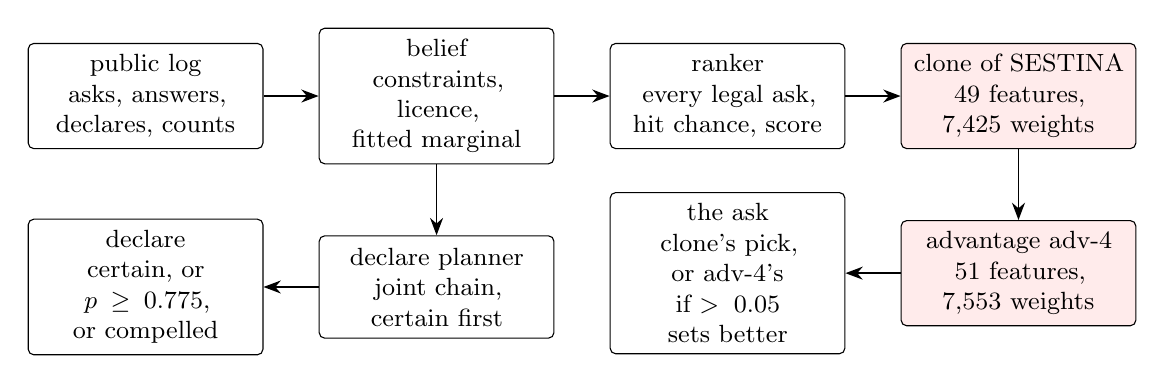
\begin{tikzpicture}[
  node distance=5mm and 7mm,
  box/.style={draw, rounded corners=2pt, align=center, font=\small, inner sep=4pt, text width=27mm, minimum height=13mm},
  hot/.style={box, fill=red!8},
  arr/.style={-{Stealth[length=2.2mm]}, semithick}]
  \node[box] (log) {public log\\asks, answers,\\declares, counts};
  \node[box, right=of log] (belief) {belief\\constraints, licence,\\fitted marginal};
  \node[box, right=of belief] (rank) {ranker\\every legal ask,\\hit chance, score};
  \node[hot, right=of rank] (clone) {clone of SESTINA\\49 features,\\7,425 weights};
  \node[hot, below=9mm of clone] (adv) {advantage adv-4\\51 features,\\7,553 weights};
  \node[box, left=of adv] (ask) {the ask\\clone's pick, or adv-4's\\if $>0.05$ sets better};
  \node[box, below=9mm of belief] (plan) {declare planner\\joint chain,\\certain first};
  \node[box, left=of plan] (decl) {declare\\certain, or $p\ge0.775$,\\or compelled};
  \draw[arr] (log) -- (belief);
  \draw[arr] (belief) -- (rank);
  \draw[arr] (rank) -- (clone);
  \draw[arr] (clone) -- (adv);
  \draw[arr] (adv) -- (ask);
  \draw[arr] (belief) -- (plan);
  \draw[arr] (plan) -- (decl);
\end{tikzpicture}
\caption{How Monet v1.0 decides. Every stage reads only public information. The two shaded stages are
learned; everything else is hand-written. Nothing is simulated at play time.}
\label{fig:pipeline}
\end{figure}

\subsection{Belief}

Monet keeps, for every unseen card, the set of seats that can still hold it: a card leaves a seat's
candidates when the seat is asked for it and misses, when it is seen elsewhere, or when the seat's hand
is full of known cards. The licence adds weight to the asker's holding of the half-suit, at
\code{licenceLambda}. Under \code{pModel:~'marginal'} (v0.4a) the constraints become a card-by-seat
probability table fitted by iterative proportional fitting, so each seat's row sums to its hand size and
each card's column to one. Under \code{pAssignment:~'joint'} (v0.4b) the declare planner places a set's
open cards by a chain over that table, most certain first, and a plan's probability is the product of
the conditionals rather than of the marginals. The belief is the work of v0.3 to v0.4c; every later
attempt to improve it measured at or below zero (\sect\ref{sec:negatives}).

\subsection{The ranker}

The hand-written ranker lists every legal ask with its hit probability $p$ and a score,
\[
  70\,p \;+\; 18\cdot\text{progress} \;+\; 12\cdot\text{narrowing} \;+\; 20\cdot\text{certain} \;+\; \text{gamble},
\]
where \emph{progress} is the fraction of the half-suit already certainly on the asker's team,
\emph{narrowing} is how much a miss would narrow the card's candidate seats ($1/(n-1)$ when the target
is one of $n$ candidates), \emph{certain} marks a sure hit, and Punter's \emph{gamble} bonus of $25$ is
paid when a hit would complete the set. Before v0.30
the ranker's argmax was the ask; from v0.30 on, the ranker only lists the asks and its numbers become
features of the learned stages.

\subsection{The clone of SESTINA}

The ask is chosen by \code{sestina-clone-3}, a model of SESTINA's own choices (\monet{} \sect{3.8ac},
\sect{3.8af}). Each legal ask is described by $49$ public features: $33$ from the ranker and the log
(the hit probability and its certainty, the ranker's relative score and rank, the half-suit's picture
by side and by target, the target's hand, who opened the half-suit, whether the card was asked before,
the seat's run and last target, and the state of the game), and $16$ that hand the model the stack's
own belief and the target's dealings with the half-suit (the slot prior, an independent per-card
probability, the target's unknown slots, and the asks, hits, misses and transfers at the target in the
half-suit and how long ago). A multilayer perceptron of width $64\cdot64$ ($7{,}425$ weights) scores
each ask as a conditional logit over the legal set, and the choice is the argmax. It was fitted on
$1{,}160{,}665$ of SESTINA's ask decisions from the bridge records (a $5\%$ sample), and it agrees with
SESTINA's choice on $58.51\%$ of held-out decisions, against $56.56\%$ for the same network on the
first $33$ features and $43.73\%$ for the stack's own choice. The fit says what SESTINA
does: it keeps asking into the half-suit it or its partner asked into before, at the target it asked
last, from the smaller hands, and it takes a certain hit for its probability and no more
(\monet{} \sect{3.8ac}).

\subsection{The learned advantage}

The clone arrives at SESTINA and stops there, so the last stage is trained on what \emph{wins} rather
than on what SESTINA chose (\monet{} \sect{3.8aw}--\sect{3.8az}). The data are paired play-outs from
the true deal: at a sampled ask decision of a self-play game, the clone's ask and an alternative are
each played to the end under one random key, and the label is the difference in the asking team's
final set differential. Each pair sets the ask actually played against one alternative: the
clone's next three, the ranker's top two, three at random, and --- in the later rounds --- the previous
model's own best, so that the model is corrected exactly where it over-rates. \code{adv-4} saw $3{,}025{,}321$ such pairs
at $554{,}197$ decisions of $32{,}000$ self-play games, in rounds at the own choices of adv-1, adv-2 and
adv-3. It is a $64\cdot64$ network over $51$ features --- the clone's $49$, the clone's own score
relative to its best, and whether the ask is the clone's top --- with $7{,}553$ weights, fitted with the
settings registered at adv-1 (Adam, batch $256$, learning rate $10^{-3}$, $L_2$ $10^{-5}$, $12$ epochs,
the best held-out epoch kept, every game $\equiv 0 \bmod 5$ held out).

At play, adv-4 scores every legal ask, and the clone's choice is replaced only by adv-4's best, and only
when adv-4 rates it more than $0.05$ sets above the clone's own. The margin was chosen on one half of
$8{,}000$ fresh games and scored on the other: there it gained $+0.0219$ sets a decision ($z$ $3.70$),
and it departs from the clone's choice at $38.14\%$ of decisions. Replayed through v0.53's policy, the first
cell of the v0.54 read differs at $35.9\%$ of Monet's asks.

\subsection{Declares, passes and the rest}

The declare has never been on the learned path. A seat that can place all six cards declares the set.
Below certainty Monet guesses only \emph{who} on its own team holds a card, never \emph{whether} the
team holds it: the speculative branch runs only when every open card's candidate seats are teammates,
and then only when the joint plan's probability is at least $0.775$ ($0.5$ when the game has stalled),
with at most two uncertain cards, and at $0.975$ for a set in which the seat holds no card.
When the rules compel a declaration it plays the planner's best plan, and abroad an uncertain compelled
claim is left to the host (MUSTFIX). The $0.775$ bar was priced at v0.50 against the true deal and sits
where realised correctness crosses break-even (\monet{} \sect{3.8av}). Four knobs that shipped earlier
--- \code{licenceLambda}, \code{contest}, \code{closing} and \code{closingFour} --- act on the ranker's
own choice and are therefore inert since v0.30, when the clone took that choice over. They stay in the
vector because removing them would be a new vector.

\begin{table}[t]
\centering
\small
\caption{Monet v1.0 = v0.54. Every knob, the rung that added it, and the read that shipped it (win rate
against SESTINA; paired difference over the version before, on the same fresh seeds).}
\label{tab:vector}
\begin{tabularx}{\linewidth}{@{}l>{\raggedright\arraybackslash}Xll@{}}
\toprule
knob & what it does & added & shipped on \\
\midrule
Punter at \code{hard} & Bass v2.0's style: ranker weights, declare bars $0.775$ / $0.5$ / $0.975$ & v0.1 & $27.08\%$ (the baseline) \\
\code{minHitP} $10^{-9}$ & sets aside asks that cannot hit & v0.2 & correctness; ``must not move'' \\
\code{licenceLambda} $0.3$ & licence weight on the ask's $p$ (inert since v0.30) & v0.3, v0.4c & $+1.19$ at $0.3$ vs $0.6$, 24 seeds \\
\code{pModel} \code{'marginal'} & the fitted card-by-seat table & v0.4a & $31.94\%$ (six seeds) \\
\code{pAssignment} \code{'joint'} & the declare planner's chain & v0.4b & $+0.81$; declares $97.86 \to 98.32\%$ \\
\code{contest} $0.6$ & credit for contested asks likely to miss (inert since v0.30) & v0.9 & $+4.04$, 12 of 12 \\
\code{closing} $0.5$, \code{closingFour} $2$ & credit for asks that close a set (inert since v0.30) & v0.20c & $+0.94$, 8 of 12 \\
\code{askModel} & the SESTINA clone chooses the ask & v0.30, v0.33 & $+7.24$; then $+3.64$ \\
\code{askAdvantageModel} \code{'adv-4'} & the learned override & v0.53, v0.54 & $+1.46$ (adv-2); then $+6.25$ \\
\code{askAdvantageMargin} $0.05$ & how much better the override must be & v0.54 & (as above) \\
\bottomrule
\end{tabularx}
\end{table}
\section{The ladder}
\label{sec:ladder}

Fifty-five numbered rungs separate v0.1 from the acceptance read (there is no v0.48, and v0.3, v0.5 and
v0.20 each carry more than one entry). Twelve vectors shipped; everything else was measured and
recorded whether or not it shipped. Table~\ref{tab:shipped} lists every shipped vector and the read
that shipped it, and Figure~\ref{fig:ladder} draws the line.

\begin{table}[t]
\centering
\footnotesize
\caption{Every shipped vector. \emph{Read}: win rate against SESTINA v1.0 on the rung's own fresh seeds.
\emph{Paired}: the mean per-seed difference over the named base on the same seeds, with its SE and the
seeds on which the candidate was ahead. Levels before 2026-09-04 were read before MUSTFIX and sit about
$1.3$ points low; the paired steps stand (\monet{} \sect{3.8f}).}
\label{tab:shipped}
\begin{tabular}{@{}llrlll@{}}
\toprule
version & what it added & read & paired over the base & seeds $\times$ deals & \monet{} \\
\midrule
v0.1  & Bass v2.0, unchanged              & $27.08\%$ & ---                                 & $6 \times 200$  & \sect{3.1} \\
v0.2  & dead asks set aside               & $27.21\%$ & $+0.13$ (``must not move'')        & $6 \times 200$  & \sect{3.2} \\
v0.3  & licence at $\lambda=0.6$          & $30.96\%$ & $+3.75$, 6 of 6                     & $6 \times 200$  & \sect{3.3a} \\
v0.4a & the fitted marginal               & $31.94\%$ & $+0.99$, 3 of 6 (unresolved)        & $6 \times 200$  & \sect{3.4a} \\
v0.4b & the joint declare chain           & $32.75\%$ & $+0.81$ (inside the floor)          & $6 \times 200$  & \sect{3.4b} \\
v0.4c & licence back at $\lambda=0.3$     & $35.12\%$ & $+1.19$ (SE $0.30$), 19 of 24       & $24 \times 200$ & \sect{3.4c} \\
v0.9  & the contest credit                & $38.92\%$ & $+4.04$ (SE $0.47$), 12 of 12       & $12 \times 200$ & \sect{3.8d} \\
v0.20c & the closing credits              & $41.25\%$ & $+0.94$ (SE $0.43$), 8 of 12        & $12 \times 200$ & \sect{3.8s} \\
v0.30 & the SESTINA clone                 & $48.01\%$ & $+7.24$ (SE $0.63$), 12 of 12       & $12 \times 200$ & \sect{3.8ac} \\
v0.33 & the clone's second feature set    & $51.04\%$ & $+3.64$ (SE $0.71$), 11 of 12       & $12 \times 200$ & \sect{3.8af} \\
v0.53 & the learned advantage (adv-2)     & $52.05\%$ & $+1.46$ (SE $0.52$), 8 of 12        & $12 \times 200$ & \sect{3.8ay} \\
v0.54 & adv-4 at margin $0.05$            & $58.42\%$ & $+6.25$ (SE $0.24$), 12 of 12       & $12 \times 800$ & \sect{3.8az} \\
\bottomrule
\end{tabular}
\end{table}

\begin{figure}[t]
\centering
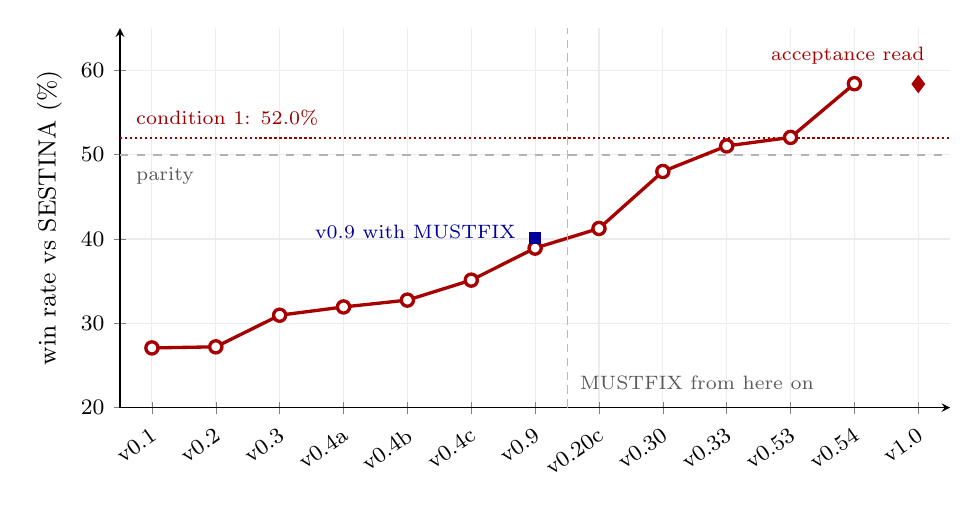
\begin{tikzpicture}
\begin{axis}[
  width=\linewidth, height=6.4cm,
  ymin=20, ymax=65, ytick={20,30,40,50,60},
  ylabel={win rate vs SESTINA (\%)},
  xmin=-0.5, xmax=12.5,
  xtick={0,...,12},
  xticklabels={v0.1,v0.2,v0.3,v0.4a,v0.4b,v0.4c,v0.9,v0.20c,v0.30,v0.33,v0.53,v0.54,v1.0},
  xticklabel style={font=\footnotesize, rotate=35, anchor=north east},
  yticklabel style={font=\footnotesize},
  ylabel style={font=\small},
  grid=major, grid style={gray!15},
  axis lines=left, clip=false]
  \addplot[gray!60, dashed, thick, domain=-0.5:12.5, samples=2] {50};
  \addplot[red!60!black, densely dotted, thick, domain=-0.5:12.5, samples=2] {52};
  \node[font=\scriptsize, gray!70!black, anchor=north west] at (axis cs:-0.4,49.6) {parity};
  \node[font=\scriptsize, red!60!black, anchor=south west] at (axis cs:-0.4,52.3) {condition 1: $52.0\%$};
  \addplot[very thick, red!65!black, mark=*, mark size=2.2pt, mark options={fill=white}]
    coordinates {(0,27.08) (1,27.21) (2,30.96) (3,31.94) (4,32.75) (5,35.12) (6,38.92) (7,41.25) (8,48.01) (9,51.04) (10,52.05) (11,58.42)};
  \addplot[only marks, mark=square*, mark size=2pt, blue!60!black] coordinates {(6,40.11)};
  \addplot[only marks, mark=diamond*, mark size=3pt, red!65!black] coordinates {(12,58.38)};
  \node[font=\scriptsize, red!65!black, anchor=south east] at (axis cs:12.25,59.6) {acceptance read};
  \node[font=\scriptsize, blue!60!black, anchor=east] at (axis cs:5.85,40.9) {v0.9 with MUSTFIX};
  \draw[gray!55, densely dashed] (axis cs:6.5,20) -- (axis cs:6.5,65);
  \node[font=\scriptsize, gray!70!black, anchor=west] at (axis cs:6.55,23) {MUSTFIX from here on};
\end{axis}
\end{tikzpicture}
\caption{Monet's win rate against SESTINA v1.0 at every shipped vector, each on its own fresh seeds.
The square is v0.9's vector re-read on the translated bridge, where every later level is read. The
diamond is v1.0 --- v0.54's vector, unchanged --- on the acceptance read's twelve fresh seeds
(\sect\ref{sec:accept}). The two steepest steps are imitation (v0.30) and the learned correction
(v0.54).}
\label{fig:ladder}
\end{figure}

\paragraph{Four phases.} The line climbed in four phases, and each was bought by a different kind of
mechanism.
\begin{enumerate}
  \item \emph{Belief, v0.3--v0.4c} ($27.08 \to 35.12\%$). Licence conditioning, the fitted marginal
        and the joint declare chain. The record's reading of the licence term is that it buys tempo,
        not accuracy: it asks into the sets the team is invested in, and its ask accuracy
        \emph{fell} ($53.84 \to 53.04\%$) while the win rate rose (\monet{} \sect{3.4c}).
  \item \emph{Ranker terms, v0.9 and v0.20c} ($\to 41.25\%$ on the translated bridge). The contest
        credit pays for asks that will probably miss into a set the opponents dominate and nobody can
        yet place. It moved $15.2\%$ of Monet's asks, cut the asks into sets its own side already held
        from $8.9\%$ to $5.9\%$, kept the turn longer ($41.7$ asks a game from $39.2$) and took the
        evenly split sets from $42.0\%$ to $46.1\%$ (\monet{} \sect{3.8d}). The idea is FishLab's own
        attribution of SESTINA, whose largest scoring component rewards exactly such asks
        \cite{fishlab}; the term is our implementation of it.
  \item \emph{Imitation, v0.30--v0.33} ($\to 51.04\%$). The clone was the largest single step of the
        ladder, $+7.24$ points ($12$ of $12$ seeds; $+7.13$ at home), and the second feature set added
        $+3.64$. Pooled over twenty-four seeds v0.33 read $50.46\%$: parity.
  \item \emph{The learned correction, v0.53--v0.54} ($\to 58.42\%$). The first advantage model, adv-2
        at margin $0.2$, changed the clone's choice at a few asks in a hundred and gained $+1.46$.
        Four times the data, a third round of labels at the model's own choices and a margin of
        $0.05$ made adv-4, which changes more than a third of the asks and gained $+6.25$ on twelve
        fresh seeds at $800$ deals ($26.5$ SE, $12$ of $12$, the lowest seed $57.31\%$), the second
        largest step. At home it won $55.76\%$ of $25{,}600$ games head to head with v0.53.
\end{enumerate}
In sets: the paired set differential moved $+0.430$ sets a game at v0.54, which the exchange rate
prices at $+5.50$ points against the $+6.25$ read. Monet's own asks hit more often ($50.69 \to 52.63\%$)
and it won more sets ($4.57 \to 4.79$ a game); the record calls these descriptions, not a mechanism.

\section{What was measured and did not ship}
\label{sec:negatives}

Most rungs shipped nothing. Table~\ref{tab:negatives} groups them by the idea they tested; the
sentences after it say what each group taught.

\begin{table}[p]
\centering
\small
\caption{The rungs that shipped nothing, grouped by idea. \emph{Abroad} is against SESTINA on twelve
fresh seeds (paired, points, $\pm 1$ SE unless marked); \emph{home} is duplicate pairs in FishAI's own
engine; a records study reads the bridge records and plays no cell.}
\label{tab:negatives}
\begin{tabularx}{\linewidth}{@{}l>{\raggedright\arraybackslash}X>{\raggedright\arraybackslash}X@{}}
\toprule
rung & mechanism & what it read \\
\midrule
\multicolumn{3}{@{}l}{\emph{Search at play time}} \\
v0.7   & determinized search, lock-only leaf, $\sim$100 ms an ask & $+0.14$ (SE $0.67$) abroad: a no-op \\
v0.28  & the search at any compute; $32$ deals (t32) & $+0.248$ a pair at home ($+3.4$ SE), then $-1.61$ (SE $0.77$) abroad \\
v0.29  & a learned leaf for the search                & eligible at home by a fifth of an SE; never read abroad \\
v0.30 M4 & the clone as the rollouts' opponents       & $-1.33$ (SE $0.74$) abroad \\
v0.36  & the clone at every seat of the rollouts      & $-1.26$ points ($-2.2$ SE) at home \\
v0.44  & the search over the clone's shortlist        & stopped at its gate: the shortlist held a hitting ask $84.0\%$ of the time and the search still chose worse \\
v0.49  & the learned leaf inside the search           & the marker against the true deal $-0.034$ (SE $0.021$); overrode a certain hit $27\%$ of the time at $-0.184$ sets each \\
v0.50  & a \emph{perfect} full-legal-set search on Monet's own belief & $-0.141$ (SE $0.102$) sets, against a hindsight ceiling of $+2.841$ \\
\midrule
\multicolumn{3}{@{}l}{\emph{Belief after v0.4c}} \\
v0.5   & opponent reading (a choice prior)            & $+0.47$ (SE $0.59$) abroad \\
v0.14--v0.15 & the assignment; the deduction fix     & records studies: both axes closed \\
v0.16  & the licence likelihood, calibrated           & $-0.74$ (SE $0.46$); wrong declares doubled through the chain \\
v0.34--v0.35 & a wider clone; a holder model of the deal & stopped at their fit gates ($+0.02$ and $-0.16$ of top-1) \\
v0.42--v0.43 & the greedy ask by the belief; its repair & the ranker's top is the greedy player, which lost to the clone by $7.24$ \\
\midrule
\multicolumn{3}{@{}l}{\emph{Ranker terms}} \\
v0.10  & a charge for hits the opponents can take back & $+1.07$ (SE $0.54$); re-read $-0.15$ (SE $0.67$) \\
v0.12--v0.13 & the closing credit by belief; a chase appetite & $-0.47$ to $-2.17$; $-1.08$ to $-7.56$ on the fit \\
\begin{tabular}[t]{@{}l@{}}v0.20b,\\ v0.22--v0.27\end{tabular} & the closing family, every rung and dose, one and two at a time & stopped at home: the shipped point is a local optimum on every axis \\
\midrule
\multicolumn{3}{@{}l}{\emph{Declaring}} \\
v0.8   & declare as soon as sampled deals agree       & $+0.08$ (SE $0.08$) abroad \\
v0.11  & a risk bar on the speculative declare        & priced on the records at a quarter of a point; not built \\
v0.32  & a clone of SESTINA's declares                & per completed set, SESTINA declares as Monet does; not built \\
v0.38  & bolder speculative claims (the holder model at the claim) & $+0.165$ a pair at home (tempo), $+0.28 \pm 0.50$ ($2$ SE) abroad \\
\midrule
\multicolumn{3}{@{}l}{\emph{Communication and learned values}} \\
v0.6   & asks chosen to reveal; the handoff           & flat or behind at home \\
v0.31  & the clone refitted wider and longer          & $+0.027$ a pair (SE $0.150$) at home \\
v0.46  & a value fitted on winning, over the clone's top~$k$ & $-0.592$ and $-0.209$ a pair at home ($8.97$ and $3.18$ SE behind) \\
v0.51  & the first advantage model (adv-1)            & its marker missed near zero ($z$ $1.01$): the winner's curse \\
\bottomrule
\end{tabularx}
\end{table}

\paragraph{Search.} Six forms of play-time search were priced, and none beat the policy it searched
over against SESTINA (\monet{} \sect{3.8a}, \sect{3.8aa}, \sect{3.8ac}, \sect{3.8ai}, \sect{3.8au}). The
one that looked best at home, where its rollouts modelled the opponents exactly, lost abroad, where
they did not. Giving the rollouts a model of SESTINA did not fix it, and neither did a better leaf:
the learned leaf predicted the end better and played worse, because it walked away from certain hits.
v0.50 then bounded the question. With the true deal, the best legal ask is worth $+2.841$ sets over
the pick at a decision; with Monet's own belief, a perfect search over every legal ask finds
$-0.141$. \emph{Hindsight is worth more than the whole ceiling}, and nothing a belief-limited search
can see is left on the table at the ask.

\paragraph{Belief.} After v0.4c the belief was studied mainly on the records, where the true deal is
known, and every route into it was priced at zero or below. The side assignment is calibrated; a
seat-known majority credit buys sure misses, not chases; and the calibrated licence likelihood, real
on the records, doubled the wrong declarations through the declare chain abroad. A pooled calibration
score could not see that selected population (\monet{} \sect{3.8j}--\sect{3.8l}).

\paragraph{Imitation caps at the imitated.} Every clone was trained to predict SESTINA's choice, so
it arrives at SESTINA and stops there; the record reached that conclusion at v0.33's parity and
tested its obvious remedy --- a selector over the clone's shortlist --- three ways (by the belief, by
search, by a value fitted on winning), and all three lost (\monet{} \sect{3.8as}). What got past parity
was not a selector over a shortlist but a correction over \emph{every} legal ask, fitted on paired
outcomes from the true deal and gated by a margin.

\paragraph{The winner's curse.} The first advantage model was right on average and wrong where it
acted: over its $53{,}263$ departures from the clone it predicted $+0.092$ sets and the true deal gave
$+0.005$. Labels at the model's own choices (a second and a third round) and four times the data are
what made the correction act on a third of the asks rather than one in seventy; the record does not
separate their contributions.

\section{What the record says about the game}
\label{sec:findings}

These are findings about \usff{} Fish between strong agents, each measured on the records or at the
bridge; the section cites where.

\begin{itemize}
  \item \textbf{One set a game is worth $12.8$ points of win rate} (\sect\ref{sec:protocol}), so a
        mechanism is worth what it moves in sets.
  \item \textbf{The position decides more than the ask.} Over v0.33's self-play, state features alone
        explain $R^2 = 0.295$ of the final set differential and the playable ask columns alone
        $0.018$; the bare scoreboard predicts the end ($R^2$ $0.248$) as well as a $24$-step rollout
        ($0.249$) (\monet{} \sect{3.8as}, \sect{3.8au}).
  \item \textbf{A hit's chance is not an ask's value.} The closing credit took asks that hit seven
        points less often and won; SESTINA leaves hits on the table and wins; hitting more is not
        evidence of playing better (\monet{} \sect{3.8c}, \sect{3.8h}, \sect{3.8as}).
  \item \textbf{A certain hit is worth keeping.} The ranker's certainty margin is worth about two
        points of win rate per point of dose (\monet{} \sect{3.8i}), and the search lost where it
        walked away from one.
  \item \textbf{Fish where the fish are.} Asks into sets the opponents dominate and nobody can yet
        place win races even when they miss (the contest credit, \sect\ref{sec:ladder}).
  \item \textbf{A split set is decided at four of six.} The first side to hold four of a 3--3 set
        converts it $56\%$ of the time between equal players; before the clone, SESTINA chased first at
        $59.4\%$ of its lead decisions where Monet's picker would have at $39.9\%$ (\monet{}
        \sect{3.8p}, \sect{3.8q}). Under the clone the gap closed: leads converted $61.1\%$ and $60.9\%$
        (\sect{3.8an}).
  \item \textbf{Declaring early buys nothing; a wrong declaration costs two.} A set the other side
        got was never a lock, because the licence rule means a lock cannot be broken; a certain set
        cashed later pays the same (\monet{} \sect{3.8f}). Monet's $0.775$ speculative bar sits where
        realised correctness crosses break-even (\sect{3.8av}), and every experiment that made Monet
        declare sooner or more boldly failed to win more games.
  \item \textbf{A hindsight oracle is not a target.} The full-information best ask is worth $+2.84$
        sets at a decision; none of it was reachable by a search on Monet's own belief. The reachable
        gain was found by learning from outcomes, not by searching the belief.
\end{itemize}
\section{The acceptance read}
\label{sec:accept}

The read was registered in \monet{} \sect{3.8ba} before any cell was played, on the owner's answer to
the proposal that closed the previous decision (\emph{``we'll go with your suggested next step''}). It
measures the shipped vector, v0.54, under the six conditions of \sect\ref{sec:protocol} exactly as
they were written, and ships nothing. The three scripts that score it were adapted from the earlier reads' and
run on those reads' cells, last written before the first cell of this read finished, and fixed by md5
before any cell was read; the runners' consoles print completion only.

\paragraph{What was played.} Twelve fresh seeds, drawn under a label written before the read against
every seed on file. On each: the arm against SESTINA v1.0 and against each of v0.2 to v0.6, and the
independently built arm against SESTINA, $200$ deals $\times$ $6$ rotations $= 1{,}200$ games a cell.
That is $84$ cells and $100{,}800$ games, played on FishLab's engine through the bridge, two containers
at a time, in about \VWallHours{} hours of wall clock. The arm plays the registry's v0.54 entry from an
export of the shipped tree, with no model file and no override, so it plays exactly what the web
build plays. Before anything else, a step-0 cell pinned the new arm to the cell that shipped v0.54
(seed 4549308, $800$ deals): every engine line but the header and the elapsed time was identical.
After the games, every recorded ask of all $84$ cells was replayed in-engine through the registry's
v0.54 entry, and every cell agreed at every ask ($72$ of $72$ for the arm, \VPinsTwin{} for the twin);
the same replay by v0.53 differs at $35.5\%$ of the asks of the cell it was run on, so the check can
see the vector.

\begin{table}[t]
\centering
\small
\caption{The six conditions of \monet{} \sect{3.9} at v0.54's vector, on twelve fresh seeds (\sect{3.8ba}).}
\label{tab:accept}
\begin{tabularx}{\linewidth}{@{}c>{\raggedright\arraybackslash}X>{\raggedright\arraybackslash}Xl@{}}
\toprule
 & condition & read & verdict \\
\midrule
C1 & $\ge 52.0\%$ against SESTINA, twelve seeds, floor $\pm 2.00$ & $58.38\%$ over $14{,}400$ games ($56.38$ to $60.38$ with the floor) & met \\
C2 & every seed $\ge 50.0\%$, SD published & lowest $56.58\%$, highest $61.17\%$, SD $1.43$ & met \\
C3 & v0.2 to v0.6 beaten, and the order monotone & $84.43 / 81.20 / 56.91 / 57.92 / 58.24$ against SESTINA's $58.38$; three ties inside the floor & met \\
C4 & declare accuracy $\ge 98.0\%$ on every cell; zero fault counters & $99.494$ to $99.857\%$ over $72$ cells; the fourteen counters zero in $2{,}587$ process files & met \\
C5 & every control of \sect{6.2}, the mirror cell excluded & the locked reader: \emph{not met} on two rows; both resolved as registered (below) & met as registered \\
C6 & reproduced by an independently built arm & \VCsixRead{} & \VCsixVerdict{} \\
\bottomrule
\end{tabularx}
\end{table}

\begin{figure}[t]
\centering
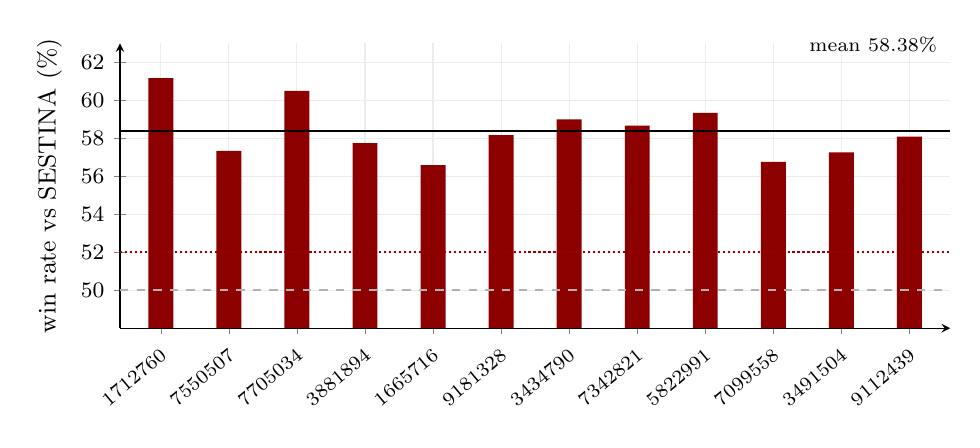
\begin{tikzpicture}
\begin{axis}[
  width=\linewidth, height=5.2cm,
  ybar, bar width=9pt,
  ymin=48, ymax=63, ytick={50,52,54,56,58,60,62},
  ylabel={win rate vs SESTINA (\%)},
  xmin=0.4, xmax=12.6,
  xtick={1,...,12},
  xticklabels={1712760,7550507,7705034,3881894,1665716,9181328,3434790,7342821,5822991,7099558,3491504,9112439},
  xticklabel style={font=\scriptsize, rotate=40, anchor=north east},
  yticklabel style={font=\footnotesize},
  ylabel style={font=\small},
  axis lines=left, grid=major, grid style={gray!15}, clip=false]
  \addplot[fill=red!55!black, draw=none] coordinates {(1,61.17) (2,57.33) (3,60.50) (4,57.75) (5,56.58) (6,58.17) (7,59.00) (8,58.67) (9,59.33) (10,56.75) (11,57.25) (12,58.08)};
  \addplot[ybar=0pt, sharp plot, gray!60, dashed, thick] coordinates {(0.4,50) (12.6,50)};
  \addplot[ybar=0pt, sharp plot, red!60!black, densely dotted, thick] coordinates {(0.4,52) (12.6,52)};
  \addplot[ybar=0pt, sharp plot, black, thin] coordinates {(0.4,58.38) (12.6,58.38)};
  \node[font=\scriptsize, anchor=south east] at (axis cs:12.55,62.0) {mean $58.38\%$};
\end{axis}
\end{tikzpicture}
\caption{The twelve seeds of the acceptance read against SESTINA v1.0, $1{,}200$ games each, in the order
they were drawn. The solid line is the mean, $58.38\%$; the dotted line is condition 1's bar for the
mean ($52\%$) and the dashed line condition 2's bar for every seed ($50\%$). The lowest seed is
$56.58\%$.}
\label{fig:seeds}
\end{figure}

\paragraph{Conditions 1 and 2.} Against SESTINA the arm won $58.38\%$ of $14{,}400$ games, with every
seed between $56.58$ and $61.17\%$ (Figure~\ref{fig:seeds}); the SE across seeds is $0.41$ points. The
shipping read of v0.54 had read $58.42\%$ on twelve other seeds at four times the deals. The stricter
reading that the record reports beside condition 1, that the floor's lower end clears $52.0\%$, holds
too. Pooled, Monet declared $4.64$ sets a game at $99.76\%$ and SESTINA $4.29$ at $96.92\%$; Monet won
$4.80$ sets a game to SESTINA's $4.20$, a differential of $+0.595$ that the exchange rate prices at
$58.06\%$.

\begin{table}[t]
\centering
\small
\caption{The panel. Twelve seeds of $1{,}200$ games per opponent. The last column is the v0.33 panel
read (\sect{3.8ar}), on twelve other seeds.}
\label{tab:panel}
\begin{tabular}{@{}lrrrrr@{}}
\toprule
opponent & mean & SD & lowest & highest & v0.33 \\
\midrule
v0.2    & $84.43\%$ & $0.80$ & $82.92$ & $85.58$ & $85.42\%$ \\
v0.3    & $81.20\%$ & $0.59$ & $80.08$ & $82.17$ & $79.28\%$ \\
v0.4    & $56.91\%$ & $1.02$ & $55.67$ & $58.67$ & $54.67\%$ \\
v0.5    & $57.92\%$ & $1.27$ & $56.00$ & $59.75$ & $54.01\%$ \\
v0.6    & $58.24\%$ & $1.26$ & $55.25$ & $60.42$ & $53.99\%$ \\
SESTINA & $58.38\%$ & $1.43$ & $56.58$ & $61.17$ & $49.87\%$ \\
\bottomrule
\end{tabular}
\end{table}

\paragraph{Condition 3.} Every older bot is beaten (Table~\ref{tab:panel}). The order is monotone only
through ties: v0.4, v0.5, v0.6 and SESTINA sit within $1.47$ points of one another, and Monet's win
rate rises slightly from v0.4 to SESTINA, the reverse of the order the condition names; every adjacent
pair is inside the $\pm 2.00$ floor, which the condition counts as a tie. The registration named this condition as the one most at risk: if the learned correction had
gained against SESTINA alone, SESTINA's column would have sat more than the floor above v0.6's and the
order would have broken. It did not. Against v0.4 to v0.6 the win rate rose from about $54\%$ at v0.33
to between $56.9$ and $58.2\%$; the seeds differ, so the comparison is not paired.

\paragraph{Condition 4.} The worst declare cell of the $72$ is $99.494\%$. The adapter's fourteen named
fault counters are zero in every one of the $2{,}587$ per-process files that were written ($5$ of
$2{,}592$ were lost to the collector: one torn, four never written); no \code{FATAL} line was
logged and no cell hit the host's move limit.

\paragraph{Condition 5, and the reader that said no.} The locked reader for \sect{6.2}'s controls
printed \emph{``CONDITION 5 NOT MET''}. Every row passed but two, and the registration had already said
how each of those is decided.
\begin{itemize}[leftmargin=*]
  \item \emph{Twelve op counts fell outside the written expectation.} The registration wrote a band for
        each op before the read and said that a miss passes only when it is located to a cause that is
        neither a defect of play nor of the instrument; the reader cannot locate, so it fails the row.
        Ten misses are \code{mustfixDeclines} against v0.2 and v0.3, whose bands came from v0.33's cells.
        The adapter counts a decline only where FishAI's rules would compel a claim and the claim is not
        certain, and the engine's own records show where that happens: v0.54's games against those two
        bots reach FishAI's dead-position rule before the clinch about $2.6$ times as often as v0.33's did
        ($0.346$ positions a game against $0.134$, and $0.118$ against $0.044$), while the declines per
        such position did not rise ($3.22 \to 3.03$ and $4.51 \to 3.41$; three is one for each of
        Monet's seats; Table~\ref{tab:located}). The
        vector moved the exposure, not the counter. The other two are SESTINA's: \code{opPoll} at one seed
        by $0.05\%$, where the count is three polls per recorded event on every cell ($2.9996$ to $2.9999$)
        and that seed played the most events; and \code{opForced} at another, the seed with the most forced
        endgames of the twelve.
  \item \emph{One cell of $72$ had no calibration file.} The text harness that prints the readout
        crashed on a cell where one of $36$ per-process files was empty. \sect{6.2} words the control
        as a per-decile readout on at least $20{,}000$ decisions on every cell, and the per-process files
        carry it: $53{,}276$ decisions on that cell, all ten deciles populated, the same bias as its
        neighbours. \sect{3.8at} scored twelve cells of the v0.33 panel, whose text harness had crashed the same
        way, as produced; the reader added the file as a requirement on a note in the registration that
        misread why those twelve files were missing (\sect\ref{sec:errata}).
\end{itemize}
The record keeps the reader's line verbatim and scores condition 5 as registered. The owner could have
held v1.0 to the reader's line instead; on 2026-09-18 they accepted condition 5 as registered
(\monet{} \sect{8.3}, row 65), so v1.0 stands.

\begin{table}[t]
\centering
\small
\caption{Where the \code{mustfixDeclines} band misses come from. \emph{Dead positions}: positions before
the clinch at which FishAI's rule for a dead game holds on the public log (no hit for $12$ events and
no claim for $24$, or no claim for $60$), counted from the engine's records. \emph{Declines}: the
adapter's count before the clinch, per complete cell.}
\label{tab:located}
\begin{tabular}{@{}llrrr@{}}
\toprule
opponent & vector & dead positions a game & declines a cell & declines per dead position \\
\midrule
v0.2    & v0.33 & $0.134$ & $517$    & $3.22$ \\
        & v0.54 & $0.346$ & $1{,}261$ & $3.03$ \\
v0.3    & v0.33 & $0.044$ & $231$    & $4.51$ \\
        & v0.54 & $0.118$ & $489$    & $3.41$ \\
v0.4    & v0.33 & $5.154$ & $16{,}455$ & $3.01$ \\
        & v0.54 & $5.366$ & $19{,}365$ & $3.01$ \\
SESTINA & v0.33 & $0.036$ & $212$    & $4.68$ \\
        & v0.54 & $0.062$ & $316$    & $4.23$ \\
\bottomrule
\end{tabular}
\end{table}

\paragraph{Condition 6.} \VCsixPara

\paragraph{The predictions.} Each condition carried a probability before the read: $97$, $95$, $65$,
$93$, $85$ and $85\%$, and about $45\%$ for all six together, most of the doubt on condition 3.
\VPredScore

\paragraph{What was seen early.} Before the readers ran, the engine lines of four of the $84$ cells had
been looked at: two v0.3 cells, in the lane log around the calibration crash, and one SESTINA cell and
one twin cell while this record was being prepared. The readers had been fixed by md5 before any of
them, and nothing in the scoring could move.
\section{Monet beside Bass, SESTINA and Kraken}
\label{sec:compare}

Table~\ref{tab:compare} sets Monet v1.0 beside the three agents it is most often compared with.
Bass v2.0 is FishAI's previous line \cite{v20}: nine hand-tuned play styles and an adaptive engine that
classifies each opponent seat from the public log and best-responds. SESTINA v1.0 is described in
\sect\ref{sec:setting}. Kraken v1.0 is the later configuration of KV's FishBot v0.6, a Python agent
that FishLab's engine runs over the same JSON protocol; its specification, as FishLab's engine source
records it, is FishBot v0.6's six parameters (\code{n\_draws} $480$ sampled deals,
\code{opponent\_gamma} $0.35$, a lookahead setting of $0.25$ with depth $3$ and beam $4$,
\code{endgame\_m} $0$) plus \code{claim\_forced\_exhaustive}, which enumerates the declaration when
one is forced. We have not played Kraken, and its column is a
description, not a measurement.

\begin{table}[t]
\centering
\small
\caption{Four agents, by what decides their asks and declarations. Monet's row is v1.0.}
\label{tab:compare}
\begin{tabularx}{\linewidth}{@{}l>{\raggedright\arraybackslash}X>{\raggedright\arraybackslash}X>{\raggedright\arraybackslash}X>{\raggedright\arraybackslash}X@{}}
\toprule
 & Bass v2.0 & SESTINA v1.0 & Kraken v1.0 & Monet v1.0 \\
\midrule
idea & adapt to the opponent & a tuned formula, and search at the end & sample deals and look ahead & learn from SESTINA, then from outcomes \\
the ask & one of nine hand-tuned styles, chosen per opponent seat & linear score over 20 features, weights by cross-entropy search; one-step lookahead & Monte Carlo over 480 sampled deals; beam lookahead, depth 3 & a clone of SESTINA's choice, overruled by a model of paired outcomes \\
search at play & none & endgame only ($\le 26$ cards unresolved): 12 deals, top 4 asks, 12 moves & every decision & none \\
declaring & style thresholds & team ownership $\ge 0.849$ and a value check & exhaustive when forced & certain first; $p \ge 0.775$; the planner's best when compelled \\
vs SESTINA & $27.08\%$ & --- & not measured & \VSestMeanPct{} (\sect\ref{sec:accept}) \\
cost & fast & not measured here & not measured & $0.178$ ms a decision \\
\bottomrule
\end{tabularx}
\end{table}

\paragraph{What each design buys.} SESTINA spends its compute where the belief is sharpest, in the
endgame, and plays a tuned linear policy elsewhere; Kraken searches every decision. Monet spends its
compute before the game: $1.16$ million imitated decisions and $3.0$ million paired play-outs,
compiled into two networks of about $7{,}500$ weights each. The record's own search results
(\sect\ref{sec:negatives}) are the argument for that choice against SESTINA: every play-time search
Monet tried was limited by its model of the other players and by its evaluation of positions, and the
learned correction was not.

\paragraph{Where Monet is weaker.} Monet does not calculate: in a forced endgame it follows its policy
where a search would enumerate. Half of its ask policy is a copy, and the copy is only as good as
SESTINA. The correction was trained on self-play with v0.33 at every seat, so an opponent unlike
anything in that population could expose it; the panel read of \sect\ref{sec:accept} is the guard
against that, and it covers five frozen FishLab releases, not people.

\section{Limitations}
\label{sec:limits}

\emph{One opponent family.} Every abroad number is against FishLab's bots in FishLab's engine; nothing
here measures play against people or against Kraken. \emph{One rule set.} \usff{} as translated into a
host that plays nine half-suits where \usff{} clinches at five; the two dialect translations (PASSFIX
and MUSTFIX) are measured and disclosed, and numbers from different bridges are never subtracted.
\emph{A second adapter, not a second engine.} Condition 6 reproduces the bridge; the engine is
FishLab's on both sides. \emph{The correction's labels.} adv-4 learned from play-outs of v0.33 in all
six seats, so the gain at home is measured against the policy its labels came from; why it carries to
SESTINA is not established by any read here. \emph{Statistical resolution.} Twelve seeds resolve
$\pm 2.00$ paired; the acceptance read is one read, and its conditions were scored once.
\emph{The ancestors are frozen.} Beating v0.2--v0.6 is evidence against having fitted SESTINA alone,
not evidence of strength.

\section{Corrections to our own record}
\label{sec:errata}

Writing this paper and reading the acceptance test found errors in \monet{}. The first two are
corrected where they stand, with the old text kept beside the correction; the last two are recorded
in the acceptance read's record (\sect{3.8ba}), beside the note they correct.

\begin{enumerate}
  \item \textbf{$+3.64$ cited for $+7.24$.} Thirteen places in \sect{3.8an}--\sect{3.8as} cite
        ``\sect{3.8ac}'s $+3.64$ at the bridge'' for the greedy ranker's loss to the clone. $+3.64$ is
        \sect{3.8af}'s read of v0.33 over v0.30; the clone over the vector before it read $+7.24$
        (\sect{3.8ac}). Every sentence argued from the direction, which stands, and no bar or decision
        was computed from the size.
  \item \textbf{SESTINA's spec keys read as its belief.} Six passages (\sect{3.8b}, \sect{3.8f},
        \sect{3.8af}, \sect{3.8ag}, \sect{3.8ah}, \sect{3.8ak}) read \code{det}, \code{cand},
        \code{depth}, \code{kappa}, \code{maxq} and \code{rbelief} as properties of SESTINA's own
        belief. They configure its endgame search (\sect\ref{sec:setting}); what the record measured
        under those names was FishAI's own mechanism and stands as such.
  \item \textbf{The calibration harness at the v0.33 panel read, unrecorded.} \sect{3.8at} scored the
        calibration readout as produced on $72$ of $72$ cells, from the per-process files, which is
        where the readout's numbers come from. Neither it nor \sect{3.8ar} recorded that the text
        harness had crashed on $12$ of those cells, each time on a per-process file that did not parse
        when it ran, so that $12$ text readouts were never written. The same crash recurred once in this
        paper's read (\sect\ref{sec:accept}).
  \item \textbf{A pre-registration note.} The note recording the acceptance read's readers said the
        condition-5 reader ``reads \code{--version}-free cover files only''; it reads every per-process
        file in each cell's cover directory and has no version filter. It also explained the reader's
        $60$ of $72$ on the v0.33 cells by twelve text files ``not on disk'', without the crash behind
        them, so the reader's calibration row did not reproduce \sect{3.8at}'s. Both sentences are
        corrected in \monet{} beside the registered text.
\end{enumerate}

\section*{Data and code}

The engine, the policy and both networks (as data modules), the probes, the tests that pin every
shipped vector and its forward bank, and \monet{} with every cell of the ladder are in the FishAI
repository. The bridge --- FishLab's engine built from source, the recording fork, the two adapters
and the game records --- is outside it, because FishLab's repository carries no licence file; it is
archived by the owner outside the public tree, and every number here can be re-read from it.

\begin{thebibliography}{9}
\footnotesize

\bibitem{monet}
FishAI project. MONET.md --- the roadmap from Monet v0.1 to v1.0. Repository document, 2026.
\S0 the target; \S3.1--\S3.4 the belief rungs; \S3.8a--\S3.8az the ladder; \S3.8ba the acceptance
read; \S3.9 the definition of v1.0; \S6.2 the controls; \S8.3 the decisions.

\bibitem{monet1}
A.~Hsieh. Toward the frontier: seventeen measured rungs against a frontier Canadian Fish agent, and
the wall where they stopped. FishAI project, 2026. The first seventeen rungs and the v0.9 acceptance
read.

\bibitem{frontier}
A.~Hsieh. Against the frontier: a cross-engine measurement and the bridge defect that nearly buried
it. FishAI project, 2026. The $27.08\%$ baseline, the mirror-cell lesson and the corrected bridge.

\bibitem{fishlab}
\code{dylann4500}. FishLab --- a Canadian Fish engine, bot family and evaluation lab. GitHub
repository, \url{https://github.com/dylann4500/FishLab}. The C++ engine, the SESTINA v1.0 frozen
specification, the v0.2--v0.6 lineage, the guest-bot protocol, the Kraken integration, and the
attribution of SESTINA's scoring terms. The repository carries no licence file; nothing from it is
reproduced here, and its measured findings are cited as its own.

\bibitem{rules}
FishAI project. RULES\_US54.md --- the ``US student'' 54-card variant. Repository rules
specification, 2026.

\bibitem{v20}
A.~Hsieh. FishAI v2.0: the three-sided ask. FishAI project, 2026. The Bass v2.0 policy Monet v0.1
forked.

\end{thebibliography}

\appendix

\section{The ladder, rung by rung}
\label{app:ladder}

Every numbered entry of \monet{}'s ladder, 2026-09-01 to 2026-09-18. \emph{Shipped} means in the
registry. Points are paired against the named base, abroad, on twelve fresh seeds unless marked.

\begin{longtable}{@{}l>{\raggedright\arraybackslash}p{0.47\linewidth}>{\raggedright\arraybackslash}p{0.33\linewidth}@{}}
\toprule
rung & idea & outcome \\
\midrule
\endhead
v0.1 & Bass v2.0 under the Monet name; the instrument & shipped: $27.08\%$ (\sect{3.1}) \\
v0.2 & dead asks set aside; two scorer fixes & shipped: $27.21\%$, ``must not move'' (\sect{3.2}) \\
v0.3 & licence conditioning at $\lambda = 0.6$; the defusal appetite frozen; score-conditioned urgency measured & shipped: $30.96\%$, $+3.75$ on six seeds (\sect{3.3}) \\
v0.4a & the fitted card-by-seat marginal & shipped: $31.94\%$, $+0.99$ unresolved (\sect{3.4a}) \\
v0.4b & the joint chain for declares & shipped: $32.75\%$, $+0.81$ (\sect{3.4b}) \\
v0.4c & the licence back at $\lambda = 0.3$ & shipped: $35.12\%$ on 24 seeds (\sect{3.4c}) \\
--- & the capability readout; the gate; the lab arm & read; ``the third row''; not built (\sect{3.5}) \\
v0.5 & opponent reading & $+0.47$ (SE $0.59$) (\sect{3.6}) \\
v0.6 & communication: revealing asks, the handoff & flat or behind at home (\sect{3.7}) \\
v0.7 & the search arm & $+0.14$ (SE $0.67$) (\sect{3.8a}) \\
v0.8 & the determinized declare & $+0.08$ (SE $0.08$) (\sect{3.8b}) \\
--- & the attribution study & read (\sect{3.8c}) \\
v0.9 & the contest credit & shipped: $38.92\%$, $+4.04$ (\sect{3.8d}) \\
v0.10 & the exposure charge & $+1.07$ (SE $0.54$); re-read $-0.15$ (\sect{3.8e}) \\
v0.11 & the declare priced; MUSTFIX adopted & $+1.28$ (SE $0.08$), a bridge correction (\sect{3.8f}) \\
--- & the majority conversion & records study (\sect{3.8g}) \\
v0.12 & the closing ask & $+0.58$ (SE $0.23$), under the floor (\sect{3.8h}) \\
v0.13 & the chase appetite & rejected on the fit (\sect{3.8i}) \\
v0.14 & the assignment & records study: the axis closes (\sect{3.8j}) \\
v0.15 & the deduction fix & records study: dead (\sect{3.8k}) \\
v0.16 & the calibrated licence likelihood & $-0.74$ (SE $0.46$) (\sect{3.8l}) \\
v0.17 & \sect{3.9} at v0.9's vector & conditions 1 and 3 not met (\sect{3.8m}) \\
--- & publication and the ship rule & the owner's rule adopted (\sect{3.8n}) \\
v0.18 & the stack read: exposure and closing & nothing clears the rule (\sect{3.8o}) \\
v0.19 & the even-set race, priced & read (\sect{3.8p}) \\
v0.20 & the four-of-six decision & read: $\Delta_{\text{lead}} = +19.6$ (\sect{3.8q}) \\
v0.20b & the race-pace term at home & stopped at home (\sect{3.8r}) \\
v0.20c & the closing credits abroad & shipped: $41.25\%$, $+0.94$ (\sect{3.8s}) \\
v0.21 & the rules-certain count & records read (\sect{3.8t}) \\
v0.22 & the closing credit at three of six & rejected at home (\sect{3.8u}) \\
v0.23 & the appetite doses moved one at a time & rejected at home (\sect{3.8v}) \\
v0.24 & the placement value & records read (\sect{3.8w}) \\
v0.25 & the trailer's ask & records read (\sect{3.8x}) \\
v0.26 & the five rung's dose above one & rejected at home (\sect{3.8y}) \\
v0.27 & the doses moved two at a time & rejected at home (\sect{3.8z}) \\
v0.28 & the search at any compute & $-1.61$ (SE $0.77$) (\sect{3.8aa}) \\
v0.29 & a learned leaf & never read abroad (\sect{3.8ab}) \\
v0.30 & the SESTINA clone & shipped: $48.01\%$, $+7.24$ (\sect{3.8ac}) \\
v0.31 & the clone refitted wider and longer & stopped at home (\sect{3.8ad}) \\
v0.32 & a declare clone & not built (\sect{3.8ae}) \\
v0.33 & the clone's second feature set & shipped: $51.04\%$, $+3.64$ (\sect{3.8af}) \\
v0.34 & the wider net at the second width & stopped at its fit gate (\sect{3.8ag}) \\
v0.35 & a holder model of the deal & stopped at its fit gates (\sect{3.8ah}) \\
v0.36 & the search with the clone as its policy & $-1.26$ points at home (\sect{3.8ai}) \\
v0.37 & the decisions the clone does not cover & records replay (\sect{3.8aj}) \\
v0.38 & the holder model in the claim path & $+0.28 \pm 0.50$ at 2 SE (\sect{3.8ak}) \\
v0.39 & where the sets go, at v0.33 & read (\sect{3.8al}) \\
v0.40 & SESTINA's gambles & read (\sect{3.8am}) \\
v0.41 & the lead conversion under the clone & read: the gap closed (\sect{3.8an}) \\
v0.42 & the belief's ceiling at our decisions & read (\sect{3.8ao}) \\
v0.43 & the repair's reach; the ceiling above the clone & read (\sect{3.8ap}) \\
v0.44 & the search over the clone's shortlist & not built: stopped at its gate (\sect{3.8aq}) \\
v0.45 & \sect{3.9} condition 3 at v0.33 & met (\sect{3.8ar}) \\
v0.46 & a value fitted on winning, over the shortlist & rejected at home (\sect{3.8as}) \\
v0.47 & \sect{3.9} conditions 5 and 6 at v0.33 & met (\sect{3.8at}) \\
v0.49 & the learned leaf inside the search & rejected at its marker (\sect{3.8au}) \\
v0.50 & the two ceilings & no belief-limited gain clears zero (\sect{3.8av}) \\
v0.51 & the learned advantage, pilot (adv-1) & its marker missed (\sect{3.8aw}) \\
v0.52 & the second round (adv-2) & held at home (\sect{3.8ax}) \\
v0.53 & adv-2 at margin $0.2$ & shipped: $52.05\%$, $+1.46$ (\sect{3.8ay}) \\
v0.54 & adv-4 at margin $0.05$ & shipped: $58.42\%$, $+6.25$ at 800 deals (\sect{3.8az}) \\
v0.55 & \sect{3.9} at v0.54's vector & \VAcceptOutcome{} (\sect{3.8ba}) \\
\bottomrule
\end{longtable}

\end{document}
